\subsection{原理・方法}

観測モデルを
\begin{align}
 y_i = f(\theta, x_i) + w_i
\end{align}
とする.加法雑音 $w_i$ は平均 $0$,観測ごとに独立,同一分布であり,共分散は有限と仮定する.
ここでは $f(\theta, x) = \phi(x)\theta$ としてパラメータに対して線形とし,最小二乗問題
\begin{align}
 \min_{\theta}\sum_{i=1}^{N}\lVert y_i - \phi(x_i)\theta\rVert^2
\end{align}
を解く.解は
\begin{align}
 \hat{\theta}_N
  = \Big( \sum_{i=1}^{N} \phi_i^\top \phi_i \Big)^{-1}
    \sum_{i=1}^{N} \phi_i^\top y_i,
 \qquad \phi_i := \phi(x_i).
\end{align}

また雑音分散が未知の場合の推定量および推定誤差共分散は
\begin{align}
 \hat{\sigma}^2
 &= \frac{1}{N-n} \sum_{i=1}^{N} \lVert y_i - \phi_i \hat{\theta}_N \rVert^2, \\
 \widehat{\mathrm{Cov}}(\hat{\theta}_N)
 &= \hat{\sigma}^2 \Big( \sum_{i=1}^{N} \phi_i^\top \phi_i \Big)^{-1}
\end{align}
で与えられる.

当てはまりの評価には決定係数
\begin{align}
 C = \frac{\sum_{i=1}^{N}\lVert \phi_i \hat{\theta}_N - \bar{y} \rVert^2}
          {\sum_{i=1}^{N}\lVert y_i - \bar{y} \rVert^2},
 \qquad
 \bar{y} = \frac{1}{N}\sum_{i=1}^{N} y_i
\end{align}
を用いる.以上は資料3.2の線形最小二乗および評価に対応する.


本実験では $\phi(x)$ として設計した特徴量から行列
\begin{align}
 X = \begin{bmatrix}
  \phi(x_1)^\top \\
  \vdots \\
  \phi(x_N)^\top
 \end{bmatrix}
\end{align}
を構成し,観測データを
\begin{align}
 y = [y_1; \dots; y_N]
\end{align}
として用いる.パラメータ推定量は
\begin{align}
 \hat{\theta} = (X^\top X)^{-1} X^\top y
\end{align}
で与えられる.

残差は
\begin{align}
 r = y - X\hat{\theta}
\end{align}
とし,雑音分散推定量は
\begin{align}
 \hat{\sigma}^2 = \frac{\lVert r \rVert^2}{N - p}
\end{align}
($p$ は列数)とする.

パラメータ推定の誤差共分散は
\begin{align}
 \hat{\sigma}^2 (X^\top X)^{-1}
\end{align}
で与えられる.

決定係数は
\begin{align}
 C = \frac{\lVert X\hat{\theta} - \bar{y}\mathbf{1} \rVert^2}
          {\lVert y - \bar{y}\mathbf{1} \rVert^2}
\end{align}
と定義する.

以下の R 関数が上記推定を実装している.

\begin{lstlisting}[language=R]
regression_simple <- function(x, y){
    theta_hat  <- solve(t(x) %*% x) %*% t(x) %*% y
    sigma2_hat <- as.numeric(t(y - x %*% theta_hat) %*%
                             (y - x %*% theta_hat) /
                             (nrow(x) - ncol(x)))
    err_cov_mat <- sigma2_hat * solve(t(x) %*% x)
    det_coef <- sum((x %*% theta_hat - mean(y))^2) /
                sum((y - mean(y))^2)
    list(theta_hat=theta_hat, err_cov_mat=err_cov_mat,
         sigma2_hat=sigma2_hat, det_coef=det_coef)
}
\end{lstlisting}


\subsection{課題1(重回帰)}

\paragraph{モデル}
$y_i = x_i^\top \theta + w_i \ (i=1,\dots,N)$.$x_i\in\mathbb{R}^2$.$w_i$ は独立,同分散 $\sigma^2$,平均0.
$X=[x_1^\top;\dots;x_N^\top]\in\mathbb{R}^{N\times2}$,$y=[y_1;\dots,y_N]\in\mathbb{R}^N$.

\paragraph{推定量}
最小二乗推定量
\[
\hat\theta_N=(X^\top X)^{-1}X^\top y .
\]
残差 $r=y-X\hat\theta_N$ により
\[
\hat\sigma^2=\frac{\|r\|_2^2}{N-p},\quad p=2, \qquad
\widehat{\mathrm{Cov}}(\hat\theta_N)=\hat\sigma^2\,(X^\top X)^{-1}.
\]
決定係数
\[
R^2=\frac{\|X\hat\theta_N-\bar y\mathbf{1}\|_2^2}{\|y-\bar y\mathbf{1}\|_2^2},\quad
\bar y=\frac1N\sum_{i=1}^N y_i .
\]

\paragraph{収束確認}
$N\in\{2,4,8,\dots,2^{13}=8192\}$ で $\hat\theta_N$ を計算し,$N$ を横軸とする片対数図で各成分を同一図に描く.

\paragraph{結果(全データ $N=10000$)}
\[
\hat\theta_{N}=
\begin{bmatrix}
1.506551\\
1.997696
\end{bmatrix},\qquad
\widehat{\mathrm{Cov}}(\hat\theta_{N})=
\begin{bmatrix}
9.866491\times10^{-5} & -4.081657\times10^{-7}\\
-4.081657\times10^{-7} & 1.005248\times10^{-4}
\end{bmatrix}.
\]
決定係数
\[
R^2=0.8629734 .
\]

\begin{figure}[H]
  \centering
  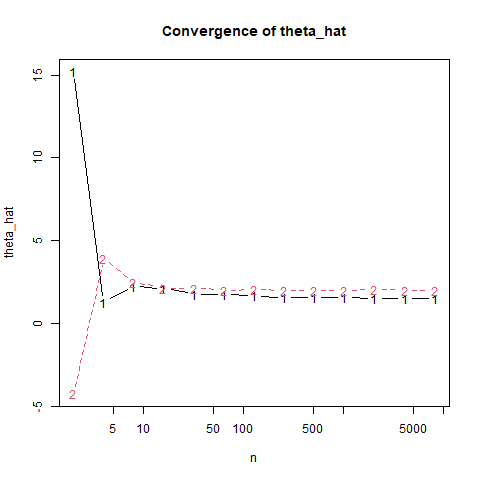
\includegraphics[width=0.75\linewidth]{graphs/task1.png}
  \caption{$\hat\theta_N$ の収束(横軸 $N=2,4,\dots,8192$ の片対数)}
  \label{fig:task1-conv}
\end{figure}

\paragraph{Rコード}
\begin{lstlisting}[language=R]
# データ読み込み
data <- read.csv("datas/mmse_kadai1.csv", header=FALSE,
                 col.names = c("x1","x2","y"))
x <- as.matrix(data[, c("x1","x2")])
y <- as.matrix(data[, "y"])

# 最小二乗(原理・方法で用いる関数)
regression_simple <- function(x, y){
  theta_hat  <- solve(t(x) %*% x) %*% t(x) %*% y
  sigma2_hat <- as.numeric(t(y - x %*% theta_hat) %*%
                           (y - x %*% theta_hat) / (nrow(x) - ncol(x)))
  err_cov_mat <- sigma2_hat * solve(t(x) %*% x)
  det_coef <- sum((x %*% theta_hat - mean(y))^2) /
              sum((y - mean(y))^2)
  list(theta_hat=theta_hat, err_cov_mat=err_cov_mat,
       sigma2_hat=sigma2_hat, det_coef=det_coef)
}

# 部分データでの実験
exp1 <- function (x, y, n){
  x <- x[1:n, , drop=FALSE]
  y <- y[1:n, , drop=FALSE]
  result <- regression_simple(x, y)
  list(theta_hat = result$theta_hat,
       err_cov_mat = result$err_cov_mat,
       det_coef = result$det_coef)
}

# 収束図の作成
plot_exp1 <- function(x, y, out="graphs/task1.png"){
  ns <- 2^(1:13)  # 2,...,8192
  theta_hats <- matrix(NA_real_, nrow=length(ns), ncol=ncol(x))
  for(i in seq_along(ns)){
    theta_hats[i, ] <- as.vector(exp1(x, y, ns[i])$theta_hat)
  }
  dir.create(dirname(out), showWarnings=FALSE, recursive=TRUE)
  png(out, width=960, height=600, res=120)
  matplot(ns, theta_hats, type="b", log="x",
          xlab="N", ylab=expression(hat(theta)),
          main="Convergence of OLS estimates")
  legend("bottomright",
         legend=paste0("theta[", 1:ncol(x), "]"),
         lty=1:ncol(x), pch=1:ncol(x))
  dev.off()
}

# 実行例(全データ)
N_max <- nrow(x)
th   <- exp1(x, y, N_max)$theta_hat
Vhat <- exp1(x, y, N_max)$err_cov_mat
R2   <- exp1(x, y, N_max)$det_coef
print(th); print(Vhat); print(R2)

# 収束図
plot_exp1(x, y)
\end{lstlisting}

\paragraph {考察}


\subsection{課題2(多項式回帰)}

\paragraph{モデル}
$y_i=\varphi(x_i)\theta+w_i,\quad \varphi(x)=[\,1\ x\ x^2\ x^3\,],\ i=1,\dots,N.$
雑音 $w_i$ は独立,同分散 $\sigma^2$,平均0.
$X=[\varphi(x_1);\dots;\varphi(x_N)]\in\mathbb{R}^{N\times4}$.

\paragraph{推定量}
推定量・共分散・決定係数は課題1と同じ形式($p=4$)で計算する.

\paragraph{収束確認}
$N\in\{4,8,16,\dots,8192\}$ で $\hat\theta_N$ を計算し,$N$ を横軸とする片対数図で各成分を同一図に描画する.

\paragraph{結果(全データ $N=10000$)}
\[
\hat\theta_N=\begin{bmatrix}
-0.50902942\\
\ \ 1.97586067\\
\ \ 0.19774405\\
-0.09866691
\end{bmatrix},\qquad
\widehat{\mathrm{Cov}}(\hat\theta_N)=\begin{bmatrix}
2.023442\times10^{-3} & -1.186497\times10^{-5} & -1.348312\times10^{-4} & \ \ 3.971165\times10^{-7}\\
-1.186497\times10^{-5} & 6.753015\times10^{-4} & -1.898545\times10^{-7} & -3.794719\times10^{-5}\\
-1.348312\times10^{-4} & -1.898545\times10^{-7} & 1.603910\times10^{-5} & \ \ 6.351820\times10^{-8}\\
\ \ 3.971165\times10^{-7} & -3.794719\times10^{-5} & \ \ 6.351820\times10^{-8} & \ \ 2.528711\times10^{-6}
\end{bmatrix}.
\]
標準誤差(対角の平方根):
$\mathrm{SE}(\hat\theta_0)\approx0.0450,\ 
\mathrm{SE}(\hat\theta_1)\approx0.0260,\ 
\mathrm{SE}(\hat\theta_2)\approx0.00400,\ 
\mathrm{SE}(\hat\theta_3)\approx0.00159.$

決定係数:
\[
R^2=0.461855 .
\]

\begin{figure}[H]
  \centering
  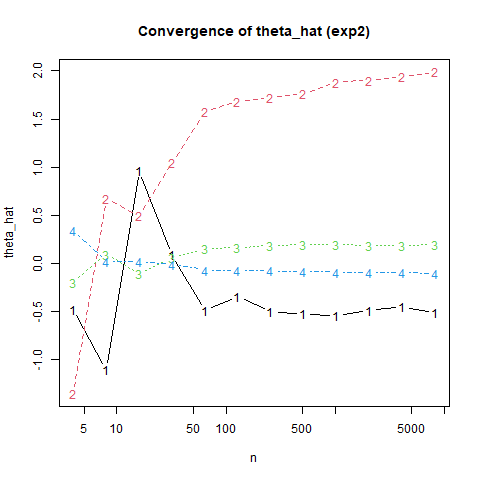
\includegraphics[width=0.75\linewidth]{graphs/task2.png}
  \caption{$\hat\theta_N$ の収束(横軸 $N=4,8,\dots,8192$ の片対数)}
  \label{fig:task2-conv}
\end{figure}

\paragraph{Rコード}
\begin{lstlisting}[language=R]
# データ
data <- read.csv("datas/mmse_kadai2.csv", header=FALSE,
                 col.names=c("x1","y"))
x0 <- rep(1, nrow(data))
x1 <- as.matrix(data[,"x1"])
x2 <- x1^2; x3 <- x1^3
x  <- cbind(x0, x1, x2, x3)
y  <- as.matrix(data[,"y"])

# OLS 基本関数(課題1と同じ)
regression_simple <- function(x, y){
  theta_hat  <- solve(t(x) %*% x) %*% t(x) %*% y
  sigma2_hat <- as.numeric(t(y - x %*% theta_hat) %*%
                           (y - x %*% theta_hat) / (nrow(x) - ncol(x)))
  err_cov_mat <- sigma2_hat * solve(t(x) %*% x)
  det_coef <- sum((x %*% theta_hat - mean(y))^2) /
              sum((y - mean(y))^2)
  list(theta_hat=theta_hat, err_cov_mat=err_cov_mat,
       sigma2_hat=sigma2_hat, det_coef=det_coef)
}

# 部分データ実験
exp2 <- function(x, y, n){
  x <- x[1:n, , drop=FALSE]
  y <- y[1:n, , drop=FALSE]
  result <- regression_simple(x, y)
  list(theta_hat=result$theta_hat,
       err_cov_mat=result$err_cov_mat,
       det_coef=result$det_coef)
}

# 収束図
plot_exp2 <- function(x, y, out="graphs/task2.png"){
  ns <- 2^(2:13)  # 4,...,8192
  theta_hats <- matrix(NA_real_, nrow=length(ns), ncol=ncol(x))
  for(i in seq_along(ns)){
    theta_hats[i, ] <- as.vector(exp2(x, y, ns[i])$theta_hat)
  }
  dir.create(dirname(out), showWarnings=FALSE, recursive=TRUE)
  png(out, width=960, height=600, res=120)
  matplot(ns, theta_hats, type="b", log="x",
          xlab="N", ylab=expression(hat(theta)),
          main="Convergence of OLS estimates (poly degree 3)")
  legend("bottomright",
         legend=paste0("theta[",0:(ncol(x)-1),"]"),
         lty=1:ncol(x), pch=1:ncol(x))
  dev.off()
}

# 実行例
N_max <- nrow(x)
print(exp2(x, y, N_max)$theta_hat)
print(exp2(x, y, N_max)$err_cov_mat)
print(exp2(x, y, N_max)$det_coef)
plot_exp2(x, y)
\end{lstlisting}
\paragraph {考察}


\subsection{課題3(分散の観測誤差:Cauchy)}

\paragraph{モデルと注意}
$y_i=x_i^\top\theta+w_i\ (i=1,\dots,N)$,$x_i\in\mathbb{R}^2$.
観測誤差 $w_i\sim \mathrm{Cauchy}(0,1)$ 独立同分布.
Cauchy は二乗可積分でないため $\mathbb{E}[w_i^2]$ が存在せず,最小二乗法の通常仮定(有限分散と大数の法則)は満たされない。
よって $\sigma^2$ や $\mathrm{Cov}(\hat\theta)$ は理論上定義できない。以下の分散・標準誤差・$R^2$ は便宜的な値であり,統計的保証はない。

\paragraph{推定(形式的なOLS)}
推定量・共分散・決定係数は課題1と同じ形式($p=2$)で計算する.
ただし観測誤差が Cauchy 分布であり理論保証がないことに注意.

\paragraph{結果(全データ $N=10000$)}
\[
\hat\theta_N=
\begin{bmatrix}
2.373074\\
1.537311
\end{bmatrix},\qquad
\widehat{\mathrm{Cov}}(\hat\theta_N)=
\begin{bmatrix}
9.234588215 & -0.003642121\\
-0.003642121 & 9.264075136
\end{bmatrix}.
\]
参考:対角の平方根は
$\mathrm{SE}(\hat\theta_1)\approx 3.0388,\ 
 \mathrm{SE}(\hat\theta_2)\approx 3.0437$.
決定係数(参考値)は
\[
R^2=0.0002841468.
\]

\begin{figure}[H]
  \centering
  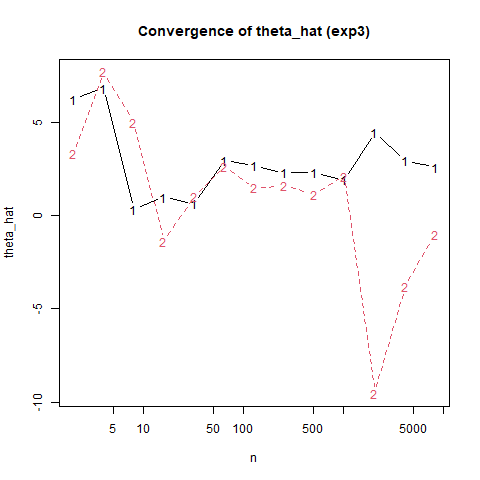
\includegraphics[width=0.75\linewidth]{graphs/task3.png}
  \caption{$\hat\theta_N$ の非収束例(横軸 $N=2,4,\dots,8192$ の片対数)}
  \label{fig:task3-conv}
\end{figure}

\paragraph{Rコード}
\begin{lstlisting}[language=R]
# データ読込
data3 <- read.csv("datas/mmse_kadai3.csv", header=FALSE,
                  col.names=c("x1","x2","y"))
x <- as.matrix(data3[, c("x1","x2")])
y <- as.matrix(data3[, "y"])

# 形式的なOLS(課題1と同様)
regression_simple <- function(x, y){
  theta_hat  <- solve(t(x) %*% x) %*% t(x) %*% y
  sigma2_hat <- as.numeric(t(y - x %*% theta_hat) %*%
                           (y - x %*% theta_hat) / (nrow(x) - ncol(x)))
  err_cov_mat <- sigma2_hat * solve(t(x) %*% x)
  det_coef <- sum((x %*% theta_hat - mean(y))^2) /
              sum((y - mean(y))^2)
  list(theta_hat=theta_hat, err_cov_mat=err_cov_mat,
       sigma2_hat=sigma2_hat, det_coef=det_coef)
}

# 部分データでの実験
exp3 <- function(x, y, n){
  x <- x[1:n, , drop=FALSE]
  y <- y[1:n, , drop=FALSE]
  res <- regression_simple(x, y)
  list(theta_hat=res$theta_hat,
       err_cov_mat=res$err_cov_mat,
       det_coef=res$det_coef)
}

# 収束図
plot_exp3 <- function(x, y, out="graphs/task3.png"){
  ns <- 2^(1:13)                      # 2,...,8192
  ns <- ns[ns <= nrow(x)]
  theta_hats <- matrix(NA_real_, nrow=length(ns), ncol=ncol(x))
  for(i in seq_along(ns)){
    theta_hats[i, ] <- as.vector(exp3(x, y, ns[i])$theta_hat)
  }
  dir.create(dirname(out), showWarnings=FALSE, recursive=TRUE)
  png(out, width=960, height=600, res=120)
  matplot(ns, theta_hats, type="b", log="x",
          xlab="N", ylab=expression(hat(theta)),
          main="Convergence of OLS under Cauchy noise")
  legend("topright", legend=paste0("theta[",1:ncol(x),"]"),
         lty=1:ncol(x), pch=1:ncol(x))
  dev.off()
}

# 実行例
N_max <- nrow(x)
print(exp3(x, y, N_max)$theta_hat)
print(exp3(x, y, N_max)$err_cov_mat)
print(exp3(x, y, N_max)$det_coef)
plot_exp3(x, y)
\end{lstlisting}

\paragraph{考察}
資料にあるように、Cauchy 誤差では外れ値の影響が支配的で,$\hat\theta_N$ は $N$ を増やしても安定しにくいことが確認できた。


\subsection{課題4(入力域の制約と設計)}

\paragraph{設定}
課題2と同じ $\varphi(x)=[\,1\ x\ x^2\ x^3\,]$, 真の $\theta$, 観測誤差 $w_i\sim\mathcal{N}(0,9)$ とする.
ただし入力は $x_i\in[0,1]$, $i=1,\dots,10000$.
$X=[\varphi(x_1);\dots;\varphi(x_N)]\in\mathbb{R}^{N\times4}$, $y=[y_1;\dots;y_N]$.

\paragraph{推定量}
推定量・共分散・決定係数は課題1と同じ形式($p=4$)で計算する.

\paragraph{Rコード}
\begin{lstlisting}[language=R]
# 課題4: x ∈ [0,1], φ(x)=[1 x x^2 x^3]
data <- read.csv("datas/mmse_kadai4.csv", header=FALSE,
                 col.names=c("x1","y"))
x0 <- rep(1, nrow(data))
x1 <- as.matrix(data[,"x1"])
x2 <- x1^2; x3 <- x1^3
x  <- cbind(x0, x1, x2, x3)
y  <- as.matrix(data[,"y"])

regression_simple <- function(x, y){
  theta_hat  <- solve(t(x) %*% x) %*% t(x) %*% y
  sigma2_hat <- as.numeric(t(y - x %*% theta_hat) %*%
                           (y - x %*% theta_hat) / (nrow(x) - ncol(x)))
  err_cov_mat <- sigma2_hat * solve(t(x) %*% x)
  det_coef <- sum((x %*% theta_hat - mean(y))^2) /
              sum((y - mean(y))^2)
  list(theta_hat=theta_hat, err_cov_mat=err_cov_mat,
       sigma2_hat=sigma2_hat, det_coef=det_coef)
}

exp4 <- function(x, y, n){
  x <- x[1:n, , drop=FALSE]
  y <- y[1:n, , drop=FALSE]
  regression_simple(x, y)
}

N_max <- nrow(x)
res4 <- exp4(x, y, N_max)
print(res4$theta_hat)
print(res4$err_cov_mat)
print(res4$det_coef)   # R^2
\end{lstlisting}

\paragraph{結果($N=10000$)}
\[
\hat\theta_{(4)}=
\begin{bmatrix}
\boxed{\text{ここに数値}}\\
\boxed{\text{ここに数値}}\\
\boxed{\text{ここに数値}}\\
\boxed{\text{ここに数値}}
\end{bmatrix},\quad
\widehat{\mathrm{Cov}}(\hat\theta_{(4)})=\boxed{\text{ここに $4\times4$ 行列}},\quad
R^2=\boxed{\text{ここに数値}}.
\]
(上の枠に,直上の R 出力を転記)

\paragraph{課題2.1との比較($N=10000$)}
課題2.1の推定結果:
\[
\hat\theta_{(2.1)}=
\begin{bmatrix}
-0.50902942\\
\ \ 1.97586067\\
\ \ 0.19774405\\
-0.09866691
\end{bmatrix},\quad
R^2=0.461855.
\]
評価観点:
\begin{itemize}\setlength{\itemsep}{0pt}
\item 分散は $\mathrm{Var}(\hat\theta)=\sigma^2(X^\top X)^{-1}$ に比例.$x\in[0,1]$ では列 $\{1,x,x^2,x^3\}$ が強く相関しやすく,$X^\top X$ の条件が悪化し $\hat\theta$ の不確かさが増えやすい.
\item $R^2$ は母集団の $y$ の散らばり($SST$)に依存.入力域が狭いと $SST$ が小さく,雑音分散が同じなら $R^2$ は低下しやすい.
\end{itemize}

\paragraph{考察(どうデータを取るべきか)}
\begin{itemize}\setlength{\itemsep}{0pt}
\item 目的は $\mathrm{Var}(\hat\theta)$ の縮小(= $X^\top X$ を「大きく」「良条件」に).
\item 入力設計:$x$ を区間全体で広く配置(例:一様),中心化・標準化して $[-1,1]$ に写像,または直交基底(Legendre/Chebyshev)で回帰.
\item 最適化観点:A/D 最適設計を用いて $\mathrm{tr}((X^\top X)^{-1})$ や $\det((X^\top X)^{-1})$ を最小化する点集合を選ぶ.
\end{itemize}
